%- 3 objects, Sequence, Primer, TestResult
%Basic in construction, all classes have toStrings and booleans.

\begin{figure}[!t]
  \begin{center}
    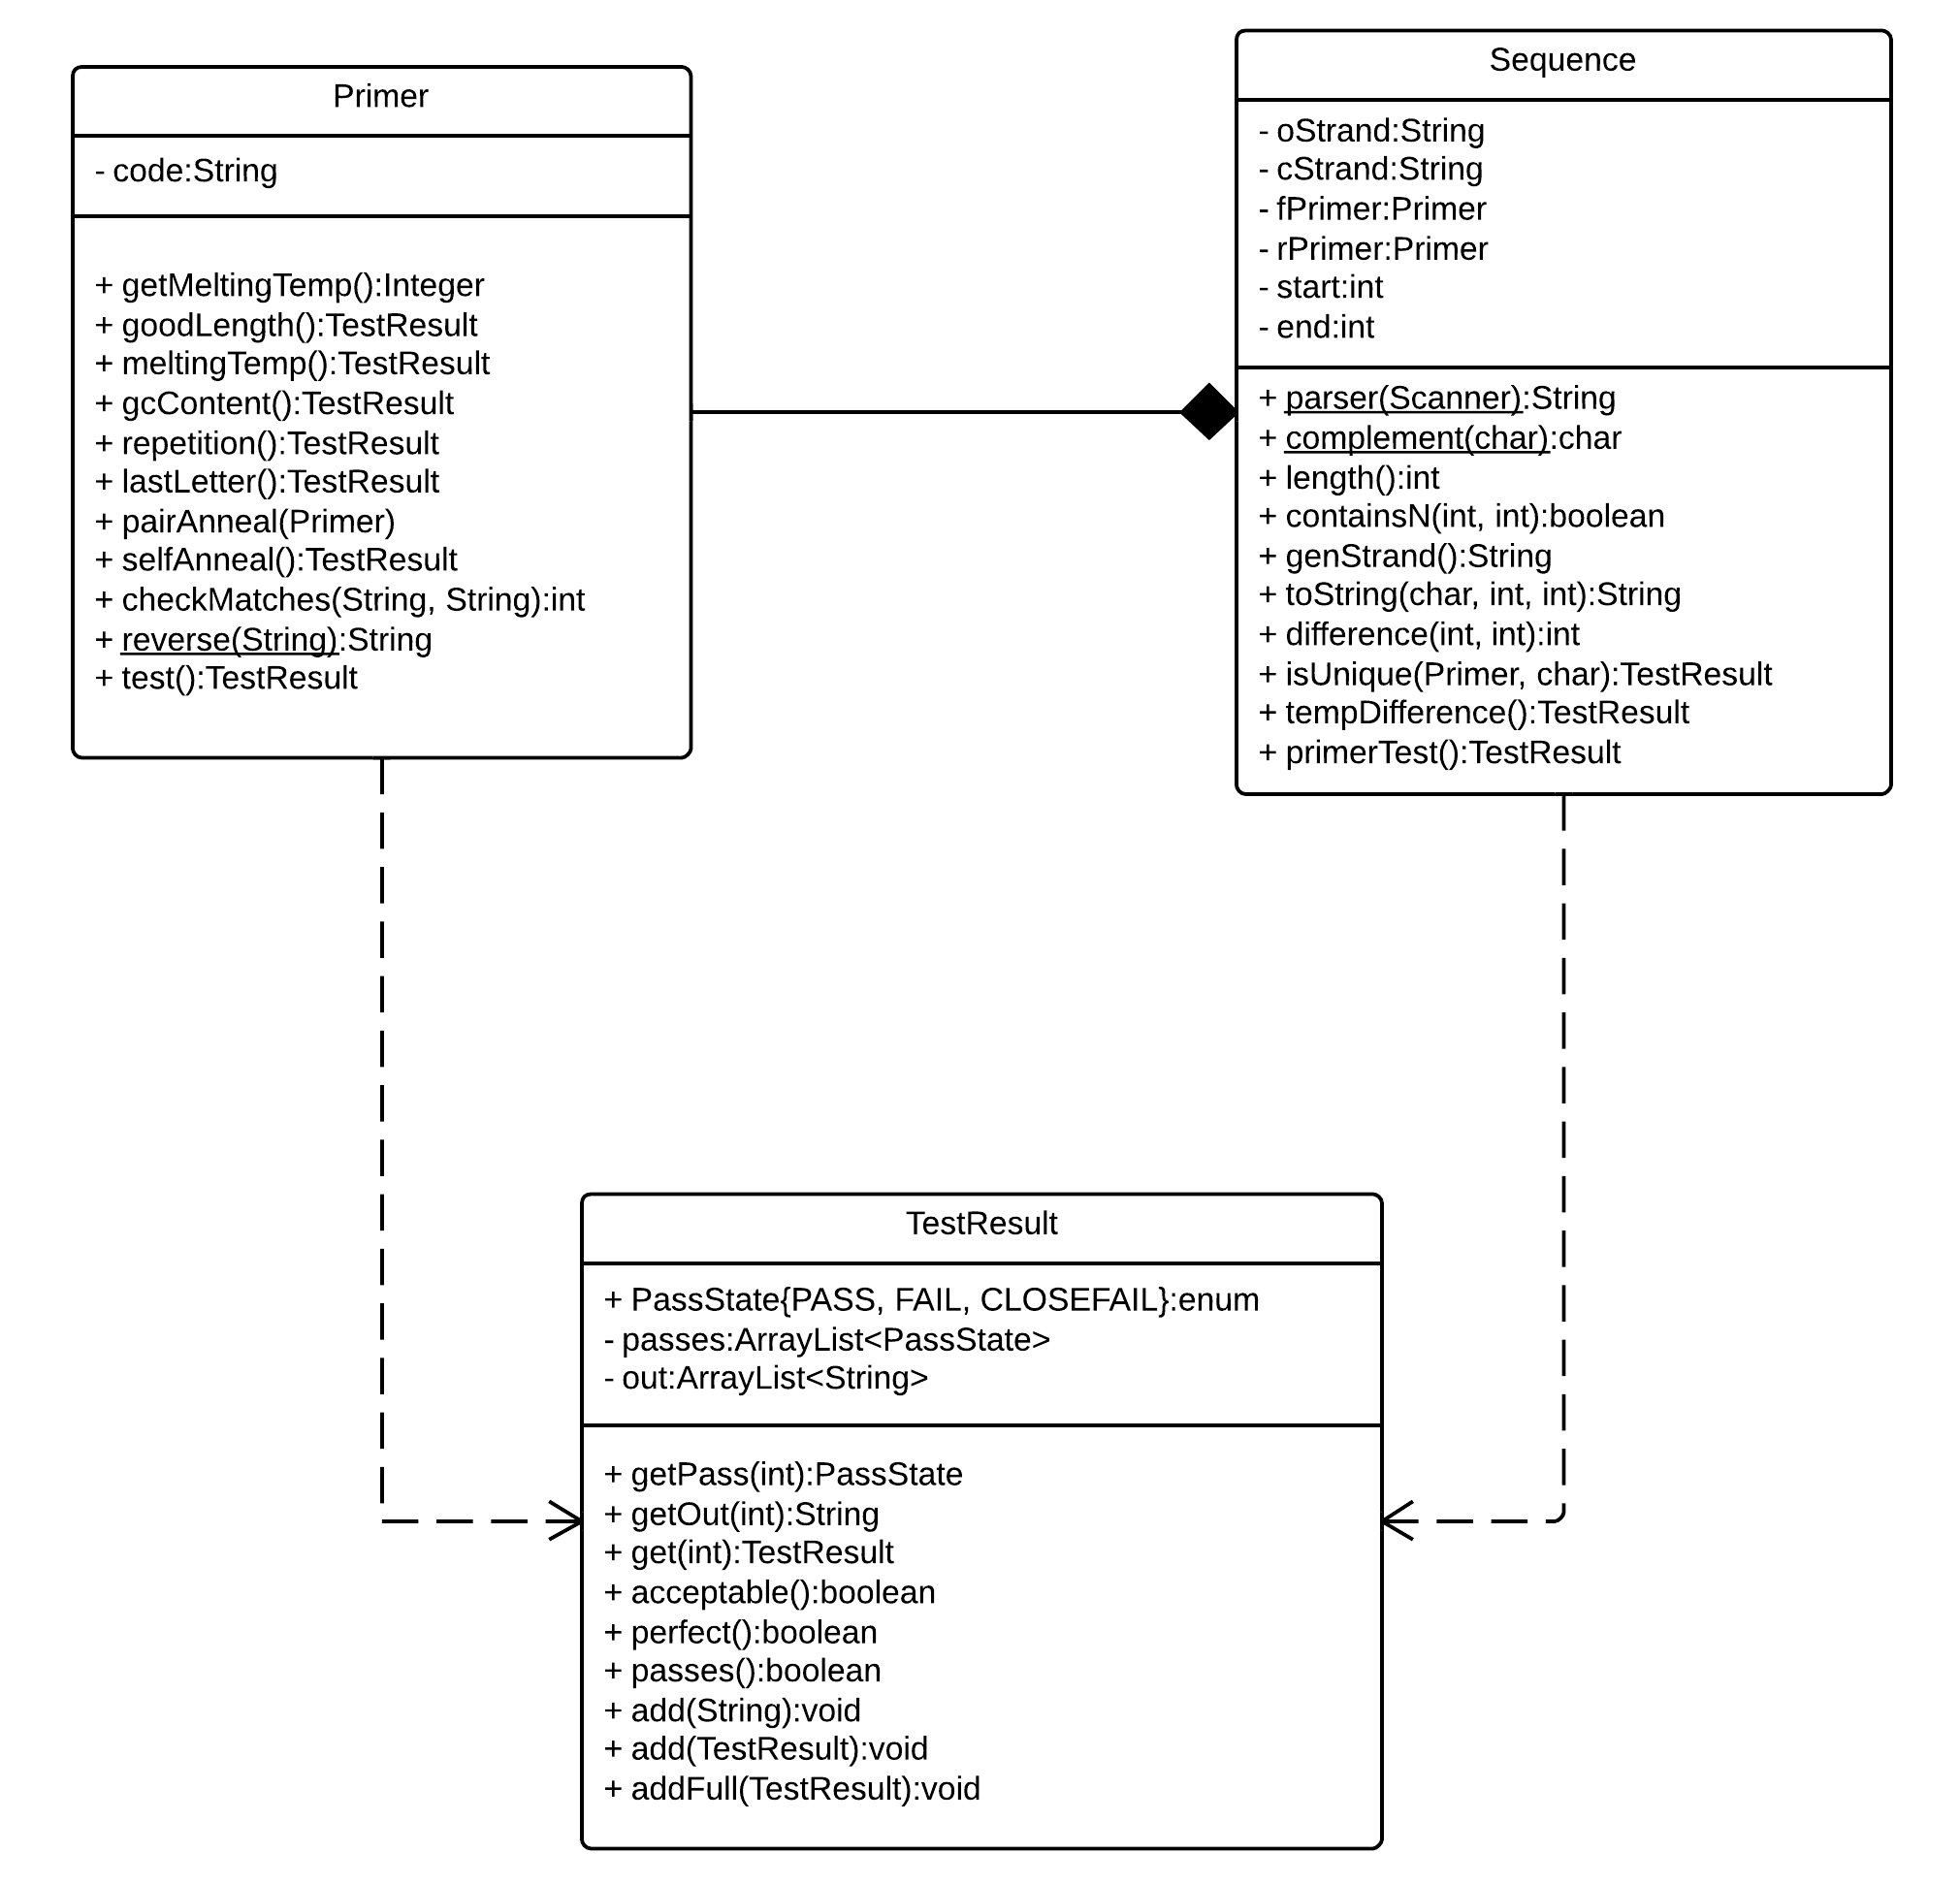
\includegraphics[width=0.75\textwidth]{./images/currentBuild/modelClassDiagram.png}
    \caption{
      \label{fig:currentBuild:model}
      Model Class Diagram 
    }
  \end{center}
\end{figure}

The models used in the application are few in number and very simple, BLAH BLAH BLAH BLAH

As seen in Figure \ref{fig:currentBuild:model}, we used three classes to represent the data:
Primer, TestResult and Sequence.

\paragraph{Primer}
The Primer class is purely designed to test user-designed primers. It has 
one instance variable, \texttt{code}, the String representing a primer
which is tested against the primer test methods, which make up the 
remainder of the class. The class is primarily made up of methods 
designed to test \texttt{code} against the various rules described in Section 
\ref{intro:prelims}. The method \texttt{test()} runs all above test 
methods and returns a TestResult indicating if the user's Primer 
is adequate without testing it against the opposing primer or its position
in the sequence as a whole.

\paragraph{TestResult}
TestResult is a class used to format the output of one or multiple primer 
tests. TestResult uses an enumerated type called PassState with values
\texttt{PASS}, \texttt{FAIL} and \texttt{CLOSEFAIL}, the last of which describes 
a state where the primer's value from a test lies outside of the recommended
values, but is within around 10\% to a pass (in most cases)and as such is seen as
acceptable, provided this is 
only the state of a minority of tests. TestResult uses two ArrayLists, one of
PassStates (\texttt{passes}) and another of Strings (\texttt{out}), to keep track 
of the state and informative message to be displayed to the user for each 
test. 

Its methods are concerned with concatenating results into larger 
TestResults. \texttt{perfect()} will return true if all entries in 
\texttt{passes} equal a \texttt{PASS}. \texttt{adequate()} will return true if the
primer follows a requisite number of general design rules (60\%) to function 
sufficiently, and is checked when deciding if a user can progress past the
primer selection stage of the exercise.
 
\paragraph{Sequence}
This class contains two Strings, \texttt{oStrand} and \texttt{cStrand}, 
representing the strand of DNA that the user entered and the ''complementary''
strand that is generated by the \texttt{parser()} method (described below)
when the sequence is constructed. Integers \texttt{start} and \texttt{end} represent 
the indexes of the start and end of the selected area in the sequence, and Primers 
\texttt{fPrimer} and \texttt{rPrimer} are representations of the user's forward
and reverse primers, respectively.
 
\texttt{parser()} is used for both sequence entry and primer input, by taking in
a String and returning a new String with all non-\texttt{atgc} characters removed.
\texttt{complement()} is a very simple function used throughout the application
that takes in one character representing a base, and returns its complement, i.e.
\texttt{complement('a')} would return \texttt{t}. \texttt{isUnique()} and \texttt{
tempDifference()} check the user's primers against their place in the larger sequence
and the difference in their temperatures. \texttt{primerTest()} uses all other test 
methods to return a TestResult that will ultimately decide if the user's primer is
adequate.  																										% phrasing?
